\section{Performance analysis}
\subsection{Datasets used}
Here is the list of the datasets used in the benchmark.\\
- imageSets/P170B328\_ServieresV\_L3\_smallest.json\\
- imageSets/P170B328\_ServieresV\_L3\_xxsmall.json\\
- imageSets/P170B328\_ServieresV\_L3\_0001-0003.json\\
- imageSets/P170B328\_ServieresV\_L3\_0001-0012.json\\
- imageSets/P170B328\_ServieresV\_L3\_0001-0024.json\\
- imageSets/P170B328\_ServieresV\_L3\_0001-0064.json\\
- imageSets/P170B328\_ServieresV\_L3\_0001-0128.json\\
- imageSets/P170B328\_ServieresV\_L3\_0001-0512.json\\
- imageSets/P170B328\_ServieresV\_L3\_0001-1024.json\\
- imageSets/P170B328\_ServieresV\_L3\_0001-2500.json\\

The two first datasets contains images (in .jpg) of 9 pixels ($3px \times 3px$). The first one only contains 1 image, and the second one contains 19 images.\\
It only took \textbf{43.1879 ms} to a single thread to get the average value.\\
\\
The other sets contain images (still in .jpg) in 4K ($3840px \times 2160px$). The smaller set contains 3 images, and the bigger one contains 2 500 images.\\
It takes \textbf{151.636 seconds} to a single thread to compute the average color of the latter sequence.\\

\subsection{Benchmark results}
This benchmark has been executed on a cluster of 3 computers (listed in the hostfile):\\
 - Manager : i7-7500U (4 cores) @ 3.5GHz with 7840 MiB of RAM\\
 - Worker1 : Celeron (4 cores) @ 2.6GHz with 3259 MiB of RAM\\
 - Worker2 : Celeron (4 cores) @ 2.2GHz with 3724 MiB of RAM\\
The operating system is Ubuntu 20.04.6 LTS x86\_64 on each computer. Computers were connected between them by Wi-Fi network.\\
\\
In order to distribute the work among processors the more evenly possible, we used the argument \emph{$--$map$-$by node} in mpirun. This way, it starts processes in a round-robin fashion accross all the computers of the hostfile. In our case, if we had for instance 8 processes, they would be distributed as shown below:\\
- Manager : Processes 1, 4, 7\\
- Worker1 : Processes 2, 5, 8\\
- Worker2 : Processes 3, 6\\
\\
The following graphs are the same, but the second one is zoomed and crop to better see the variations on the small image sets.
\begin{figure}[H]
    \centering
    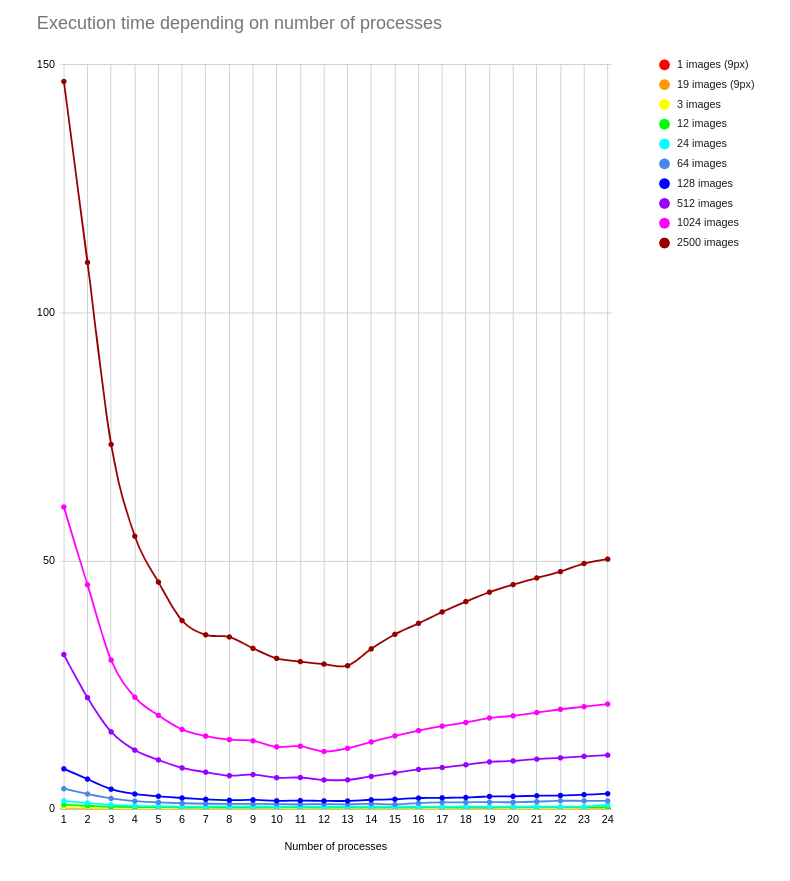
\includegraphics[width=8.2cm]{images/perfsAverage.png}
    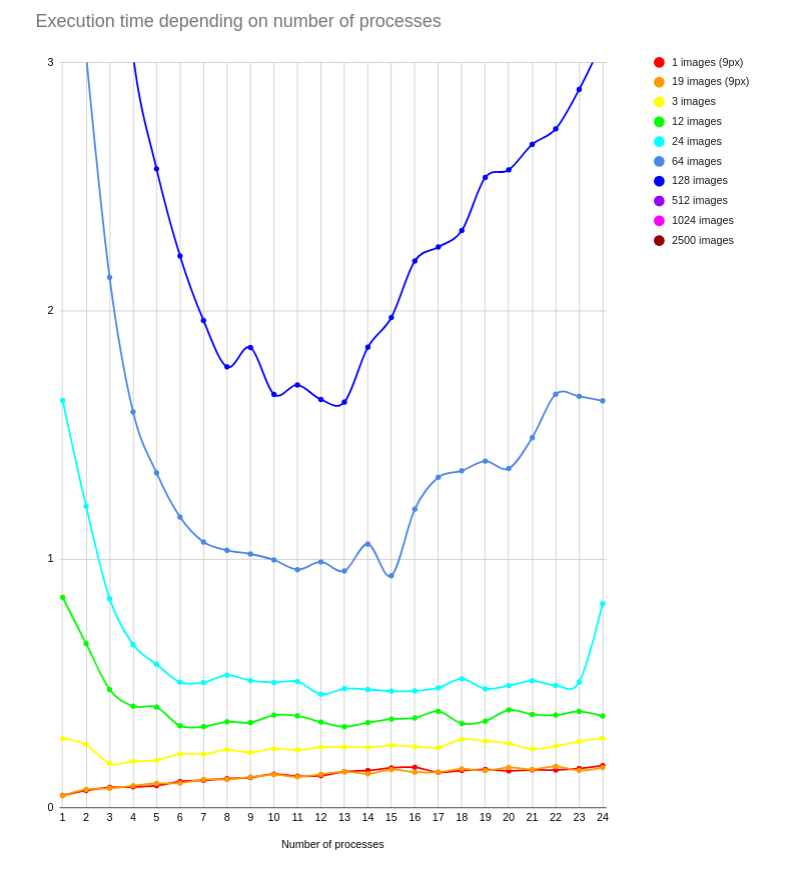
\includegraphics[width=8.2cm]{images/perfsAverageZoomed.png}
    \caption{Results from benchmark}
    \label{fig:benchmarkResAverage}
\end{figure}
In these graphs, we plotted the calculations' duration (in seconds) depending on the number of processes available. We tested it for each dataset.\\
The values here are average values, each configuration has been tested 6 times.\\
You can see below the exact values for each test.

\begin{figure}[H]
    \centering
    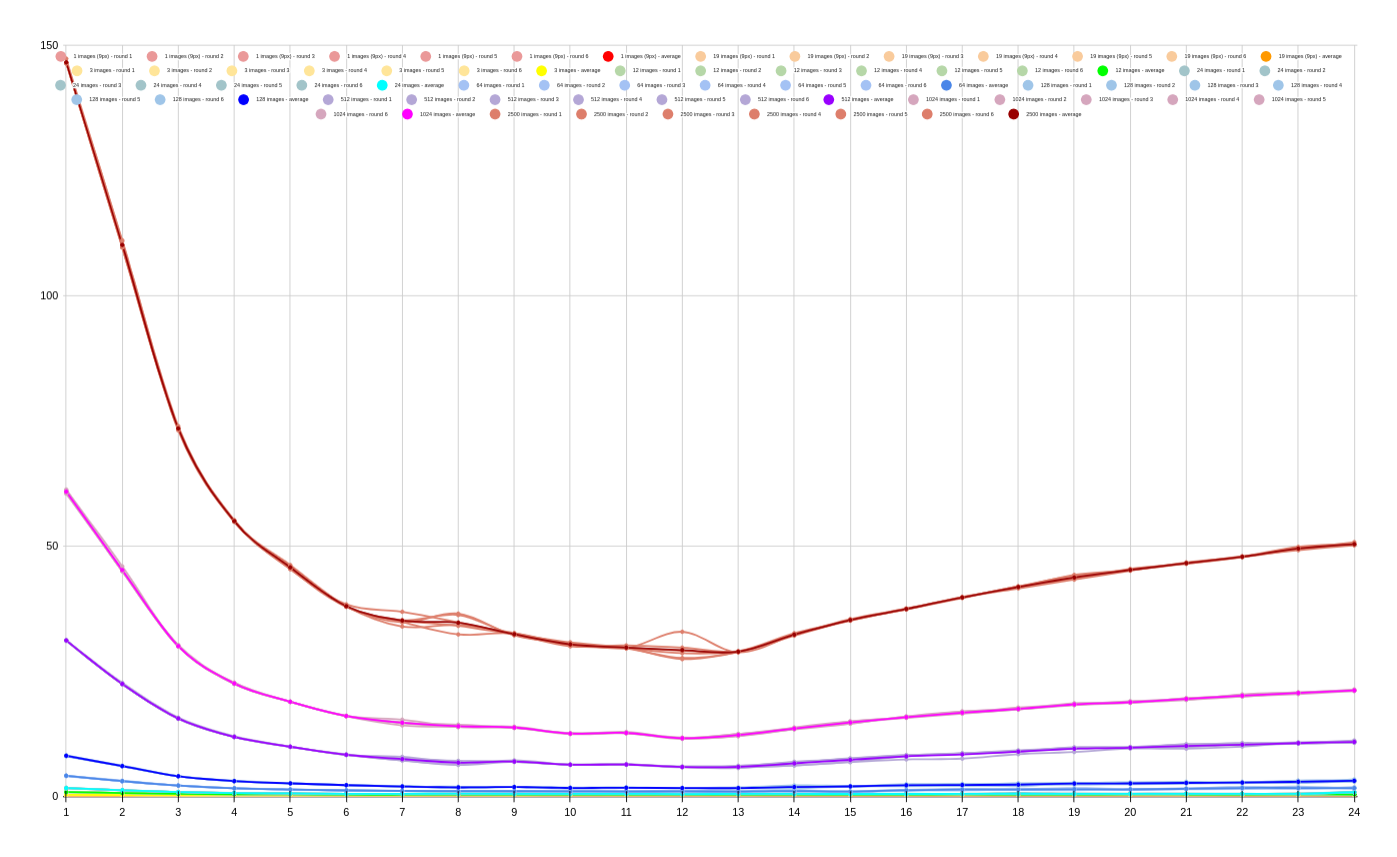
\includegraphics[width=18cm]{images/perfsAll.png}
    \caption{Results from benchmark}
    \label{fig:benchmarkRes}
\end{figure}
\begin{figure}[H]
    \centering
    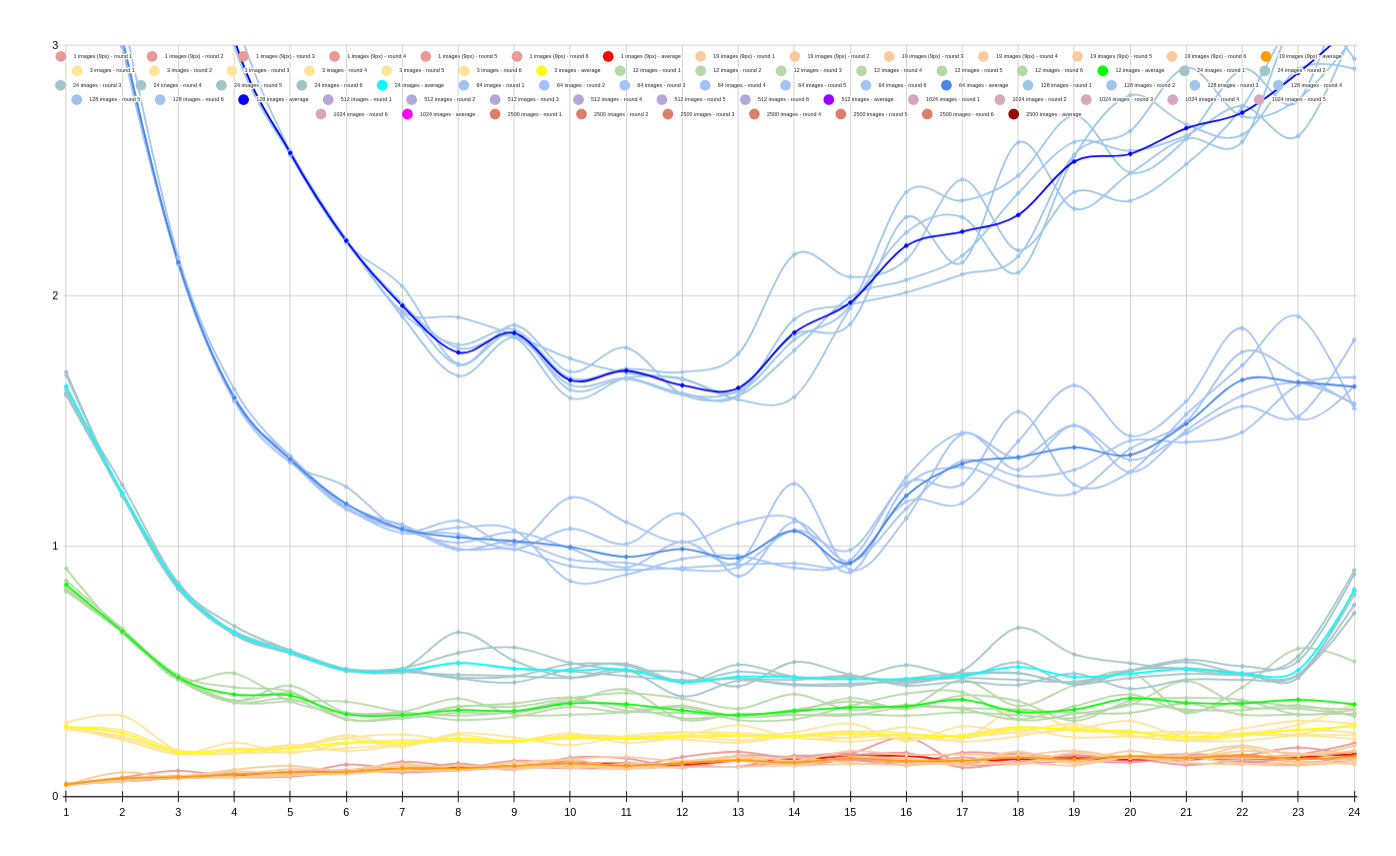
\includegraphics[width=18cm]{images/perfsAllZoomed.png}
    \caption{Results from benchmark}
    \label{fig:benchmarkResZoomed}
\end{figure}
As we can see if the calculations are too simple, it is better to spawn only one process.
For bigger sets, which need more calculations, we can see that the best number of procresses is around 12.

\subsection{Explanations}
MPI introduce a new latency, the network. Indeed, to communicate information with the other computers of the cluster, MPI needs to send requests, communicate with ssh... and this take more time than just executing the calculations on a single thread without communicating anything.\\
So if the dataset is too small (< number of cores of the cluster), and/or if the images of the set are too small (only few pixels), it is quicker to use a single thread.\\
\\
For bigger datasets, we can see that the minimum of calculations' duration is obtained when the number of processes is around 12.\\
This is normal because it is the total number of cores of the cluster (4 + 4 + 4 = 12).\\
If we start fewer processes, then we do not use the processors at 100\% of their capacity, so it will be less efficient.\\
Otherwise, if we start more processes, then we don't have "perfect" parallelism. Processors of each computer have to do context switching between all processes as there are more active processes than cores available to run them. This slows down calculations.